% \documentclass[aspectratio=169,notes]{beamer}
\documentclass[aspectratio=169]{beamer}
\usetheme[faculty=phil]{fibeamer}
\usepackage{polyglossia}
\setmainlanguage{english} %% main locale instead of `english`, you
%% can typeset the presentation in either Czech or Slovak,
%% respectively.
\setotherlanguages{russian} %% The additional keys allow
%%
%%   \begin{otherlanguage}{czech}   ... \end{otherlanguage}
%%   \begin{otherlanguage}{slovak}  ... \end{otherlanguage}
%%
%% These macros specify information about the presentation
\title[MaM]{Mechanics and Machines, CAD Details 2} %% that will be typeset on the
\subtitle{Workflow, Work in groups
\\ CAD file formats \\ Threads
         } %% title page.
\author{Oleg Bulichev}
%% These additional packages are used within the document:
\usepackage{ragged2e}  % `\justifying` text
\usepackage{booktabs}  % Tables
\usepackage{tabularx}
\usepackage{tikz}      % Diagrams
\usetikzlibrary{calc, shapes, backgrounds}
\usepackage{amsmath, amssymb}
\usepackage{url}       % `\url`s
\usepackage{listings}  % Code listings
% \usepackage{subfigure}
\usepackage{floatrow}
\usepackage{subcaption}
\usepackage{mathtools}
\usepackage{todonotes}
\usepackage{fontspec}
\usepackage{multicol}
\usepackage{pdfpages}
\usepackage{wrapfig}
\usepackage{animate}
\usepackage{booktabs}
\usepackage{multirow}
% \usepackage{graphicx}
\usepackage{colortbl}

\graphicspath{{resources/}}
\frenchspacing

\setbeamertemplate{caption}[numbered]
\usetikzlibrary{graphs}

% \usepackage[backend=biber,style=ieee,autocite=footnote]{biblatex}
% \addbibresource{biblio.bib}
% \DefineBibliographyStrings{english}{%
%   bibliography = {References},}

\newcommand{\oleg}[2][] {\todo[color=red, #1] {OLEG:\\ #2}}
\newcommand{\fbckg}[1]{\usebackgroundtemplate{\includegraphics[width=\paperwidth]{#1}}}%frame background

\usepackage[framemethod=TikZ]{mdframed}
\newcommand{\dbox}[1]{
\begin{mdframed}[roundcorner=3pt, backgroundcolor=yellow, linewidth=0]
\vspace{1mm}
{#1}
\vspace{1mm}
\end{mdframed}
}

\begin{document}
\setlength{\abovedisplayskip}{0pt}
\setlength{\belowdisplayskip}{0pt}
\setlength{\abovedisplayshortskip}{0pt}
\setlength{\belowdisplayshortskip}{0pt}

\fbckg{fibeamer/figs/title_page.png}
\frame[c]{\setcounter{framenumber}{0}
    \usebeamerfont{title}%
    \usebeamercolor[fg]{title}%
    \begin{minipage}[b][6.5\baselineskip][b]{\textwidth}%
        \textcolor{black}{\raggedright\inserttitle}
    \end{minipage}
    % \vskip-1.5\baselineskip

    \usebeamerfont{subtitle}%
    \usebeamercolor[fg]{framesubtitle}%
    \begin{minipage}[b][3\baselineskip][b]{\textwidth}
        \raggedright%
        \insertsubtitle%
    \end{minipage}
    \vskip.25\baselineskip
}
%   \frame[c]{\maketitle}

\fbckg{fibeamer/figs/common.png}

\note{\scriptsize \begin{itemize}
        \item \
    \end{itemize}}

\note{
    \begin{columns}[T,onlytextwidth]
        \begin{column}{0.39\textwidth}
            \begin{enumerate}
                \item Воркфлоу это про то где и для чего нам такие форматы нужны: проектирование и симуляция
                \item Есть видос, его надо показывать для объяснения форматов
            \end{enumerate}
        \end{column}
        \begin{column}{0.59\textwidth}
            \begin{figure}[H]
                \centering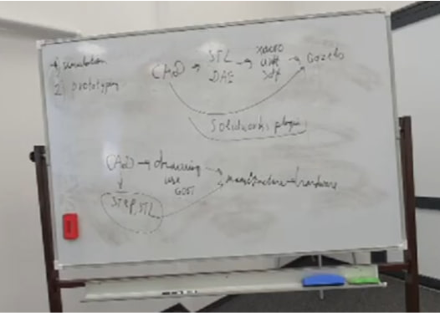
\includegraphics[height=5cm,width=1\textwidth,keepaspectratio]{helper.png}
                % \caption{caption_name}
                \label{fig:helper.png}
            \end{figure}
        \end{column}
    \end{columns}
}

\begin{frame}[c]{Workflow}
\framesubtitle{}
    \LARGE
    \centering On whiteboard
\end{frame}

\begin{frame}[t]{Popular neutral formats}
\framesubtitle{}
\Large
    \begin{itemize}
        \item step
        \item stl
        \item dae
        \item jt
    \end{itemize}
\end{frame}

\begin{frame}[t]{Stereolithography (.STL)}
\framesubtitle{}
    \begin{columns}[T,onlytextwidth]
        \begin{column}{0.59\textwidth}
            \textbf{Application:} for 3d printers, Gazebo sim

\textbf{Feature:} STL files describe only the surface geometry of a three-dimensional object without any representation of color, texture or other common CAD model attributes.

        \end{column}
        \begin{column}{0.39\textwidth}
            \begin{figure}[H]
                \centering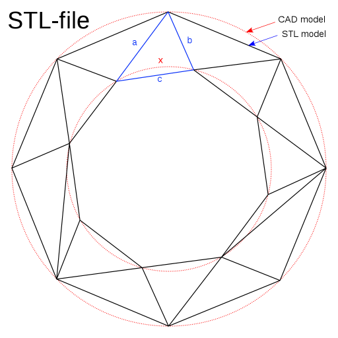
\includegraphics[height=4cm,width=1\textwidth,keepaspectratio]{stl.png}
                % \caption{caption_name}
                \label{fig:stl.png}
            \end{figure}
        \end{column}
    \end{columns}
\end{frame}

\begin{frame}[t]{ISO 10303 (.STEP)}
\framesubtitle{}
\textbf{Application:} is an ISO standard for the computer-interpretable representation and exchange of product manufacturing information

\textbf{Feature:} Does not contain a lot of information, \textit{including threads}!

\end{frame}

\begin{frame}[t]{COLLADA (.DAE)}
\framesubtitle{}
\textbf{Application:} COLLADA was originally intended as an intermediate format for transporting data from one digital content creation (DCC) tool to another application.

\textit{Blender, Maya, Meshlab}

\textbf{Feature:} XML, which contains detail + texture

\end{frame}

\begin{frame}[t]{Jupiter Tesselation (.JT)}
\framesubtitle{}
\textbf{Application:} is an openly-published ISO-standardized 3D CAD data exchange format used for product visualization, collaboration, digital mockups, and other purposes.

\textbf{Feature:} The format and associated software is structured so that extremely large numbers of components can be quickly loaded, shaded and manipulated in real-time. 

Because JT files are inherently "lightweight" ($\approx $1-10\% of the size of a CAD file) they are ideal for internet collaboration.

\end{frame}

\begin{frame}[t]{Threads and difference between formats}
\framesubtitle{Video}
    
\end{frame}

\begin{frame}[c]{Tools for group work}
\framesubtitle{}
\LARGE
\centering Grabcad Workbench or OpenBom
    
\end{frame}

\begin{frame}[t]{Task for MegaChads}
    \framesubtitle{Video}
    \vspace{-0.6cm}
    \begin{figure}[H]
        \href{https://youtu.be/LirvZRS8lRQ}{
            \centering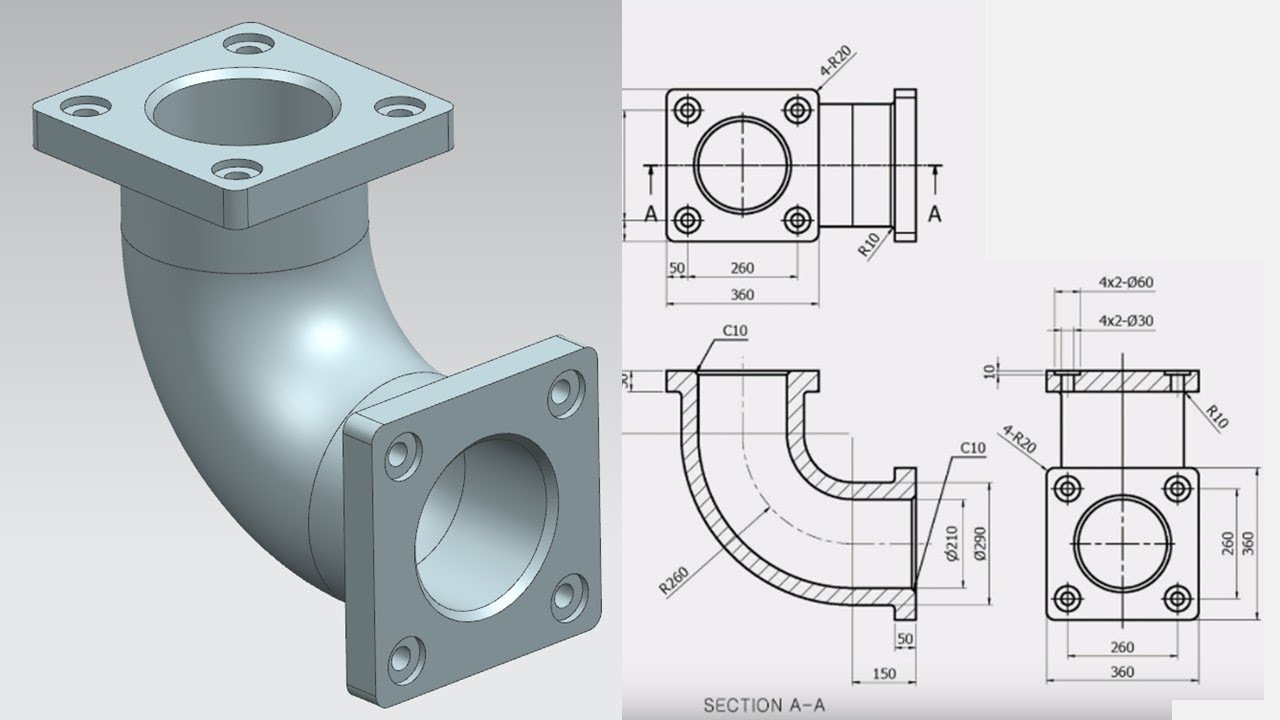
\includegraphics[height=6cm,width=1\textwidth,keepaspectratio]{megachad.jpg}}
        % \caption{Click on a picture for a video}
        \label{fig:megachad.jpg}
    \end{figure}
\end{frame}

\begin{frame}[t]{Task for GigaChads}
    \framesubtitle{Video}
    \vspace{-0.6cm}
    \begin{figure}[H]
        \href{https://youtu.be/zxm297gENnU}{
            \centering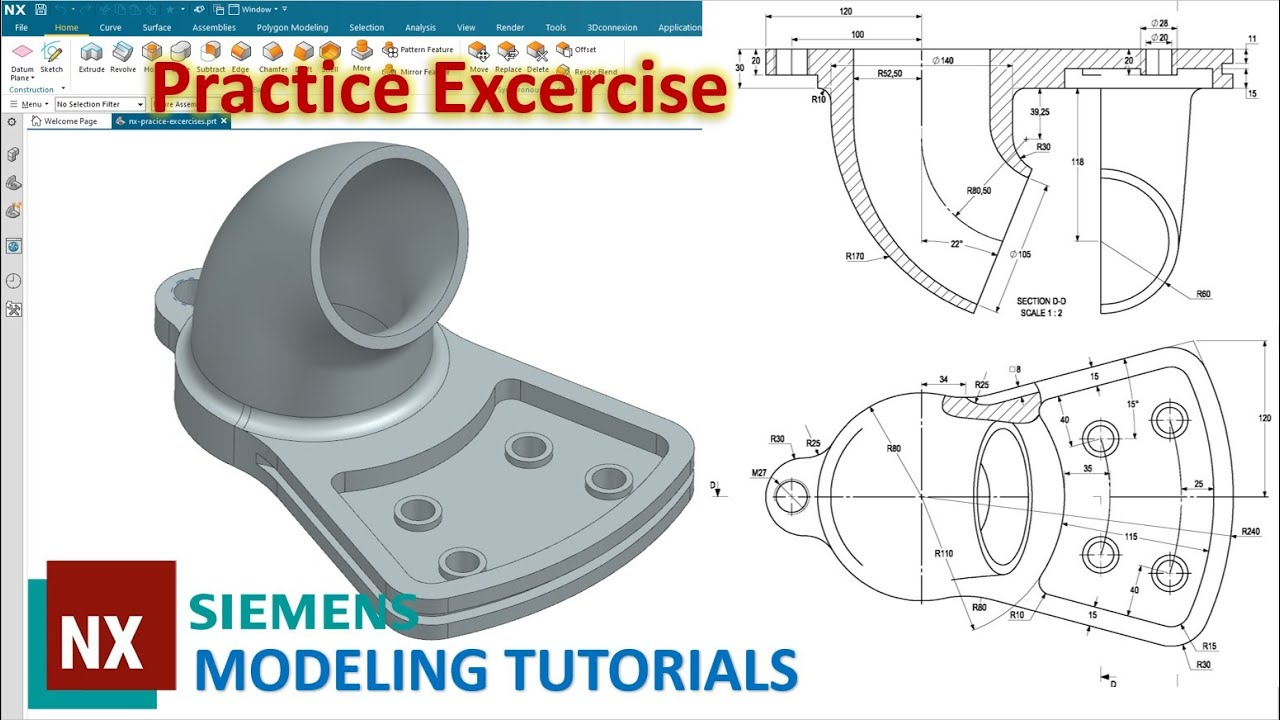
\includegraphics[height=6cm,width=1\textwidth,keepaspectratio]{gigachad.jpg}}
        % \caption{Click on a picture for a video}
        \label{fig:gigachad.jpg}
    \end{figure}
\end{frame}

\begin{frame}[t]{Task for Oleg-likeChads}
    \framesubtitle{Video}
    \vspace{-0.6cm}
    \begin{figure}[H]
        \href{https://youtu.be/Q0JvkLUzkpU}{
            \centering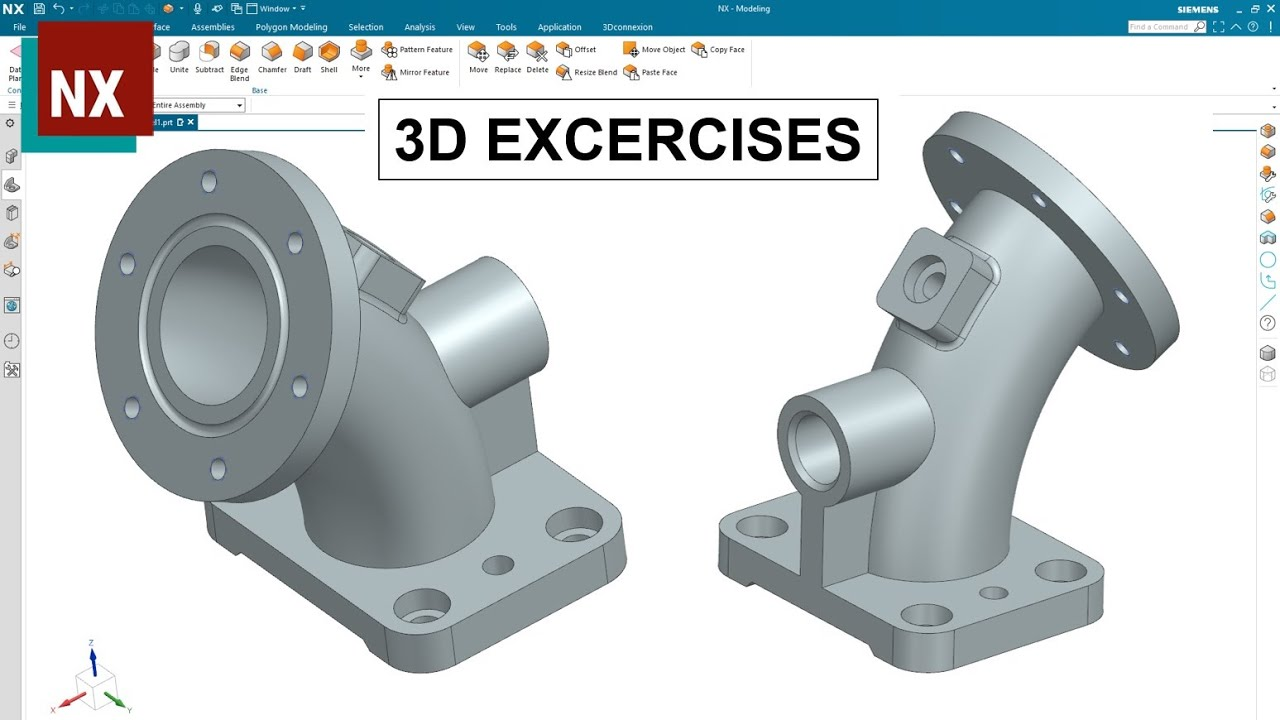
\includegraphics[height=6cm,width=1\textwidth,keepaspectratio]{olegchad.jpg}}
        % \caption{Click on a picture for a video}
        \label{fig:olegchad.jpg}
    \end{figure}
\end{frame}

% \begin{frame}[t]{Reference material}
%     % \Large
%     \begin{itemize}
%         \item \textit{"Mechanisms and Machines: Kinematics, Dynamics, and Synthesis" Michael M. Stanisic, pdf pages 21--56 } \textbf{1.1 --- 1.6}
%         \item \textit{"Theory of Machines and Mechanisms" John J. Uicker, pdf pages 33--59 } \textbf{1.4 --- 1.7}
%         \item \textit{"Design of machinery" Robert L. Norton, pdf pages 57--79 } \textbf{2.0 --- 2.11}
%         \item \textit{"Механика. Теория механизмов и машин" Конищева О. В., pdf pages 7--23 } \\ Структурный анализ и классификация плоских механизмов
%         \item \textit{"Теория механизмов и машин" Артоболевский И. И. 1988, pdf pages 21--63 } \\ Структурный анализ и классификация механизмов
%               % \item \href{https://onlinemschool.com/math/library/vector/cos/}{Direction cosines (OnlineMSchool)}
%     \end{itemize}
% \end{frame}

\fbckg{fibeamer/figs/last_page.png}
\frame[plain]{}

\end{document}